\section{Lecture 29}
\subsection{Lecture Notes - Cross Sections in Different Frames}
\subsubsection{Main Result from Last Day}
Rutherford Cross section of:
\[\dod{\sigma}{\Omega} = \frac{q_1^2q_2^2}{16E^2}\frac{1}{\sin^6\frac{\theta}{2}}\]
But so far, we have assumed that the scatterer is infinitely heavy/immobile. This is in general not the case, the target can of course move if $m_1$ is on the same mass scale as $m_2$. Today we deal with this scenario.

\subsubsection{CM vs Lab Frames}
\begin{center}
    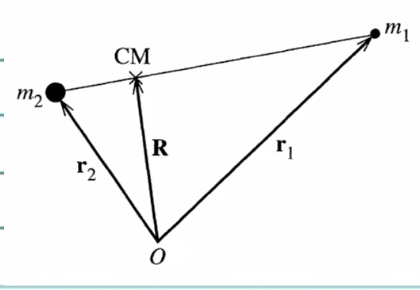
\includegraphics[scale=0.5]{Lecture-29/l29-img1.png}
\end{center}
We have two coordinates in the COM frame:
\[\v{r} = \v{r}_1 - \v{r}_2 \quad \text{(Relative coordinate)}\]
The relative coordinate moves like a single particle with reduced mass $\mu = \frac{m_1m_2}{M}$ where $M = m_1 + m_2$. The Lagrangian in this frame is given by:
\[\LL = T_{COM} + T_{rel} - U\]
\[\LL = \frac{M}{2}\dot{\v{R}}_{COM}^2 + \frac{\mu}{2}\dot{\v{r}}^2 - U(\v{r})\]
The generalized momentum $\v{p}$ is given as:
\[\v{p} = \mu \dot{\v{r}}\]
A question: What can we say of the momenta of the two particles in the COM frame?
\begin{s}
In the COM frame, it must hold that $\v{p}_1 = -\v{p}_2$ as of course the total momentum must be zero.
\end{s}
We can also see the above fact if we write:
\[\v{r}_1 = \v{R} + \frac{m_2}{M}\v{r}, \quad \v{r}_2 = \v{R} - \frac{m_1}{M}\dot{\v{r}}\]
In the CM, $\dot{\v{R}} = 0$, as the total momentum must be zero. Hence, taking the derivative of the above equations:
\[\dot{\v{r}}_1 = \frac{m_2}{M}\dot{\v{r}} \implies m_1\v{r}_1 = \frac{m_1m_2}{M}\v{r} = \v{p}\]
\[\dot{\v{r}}_2 = - \frac{m_1}{M}\dot{\v{r}} \implies m_2\dot{\v{r}}_2 = - \frac{m_1m_2}{M}\dot{\v{r}} = -\v{p}\]
What can we say about the momenta of two particles in the COM frame before (unprimed) and after (primed) an elastic collision?
\begin{s}
After the collision, since energy is conserved, the length of these vectors are conserved; hence,
\[\abs{\v{p}_1} = \abs{\v{p}'_1}, \quad \abs{\v{p}_2} = \abs{\v{p}'_2}\]
Velocities rotate, but remain colinear by momentum/energy conservation.
\begin{center}
    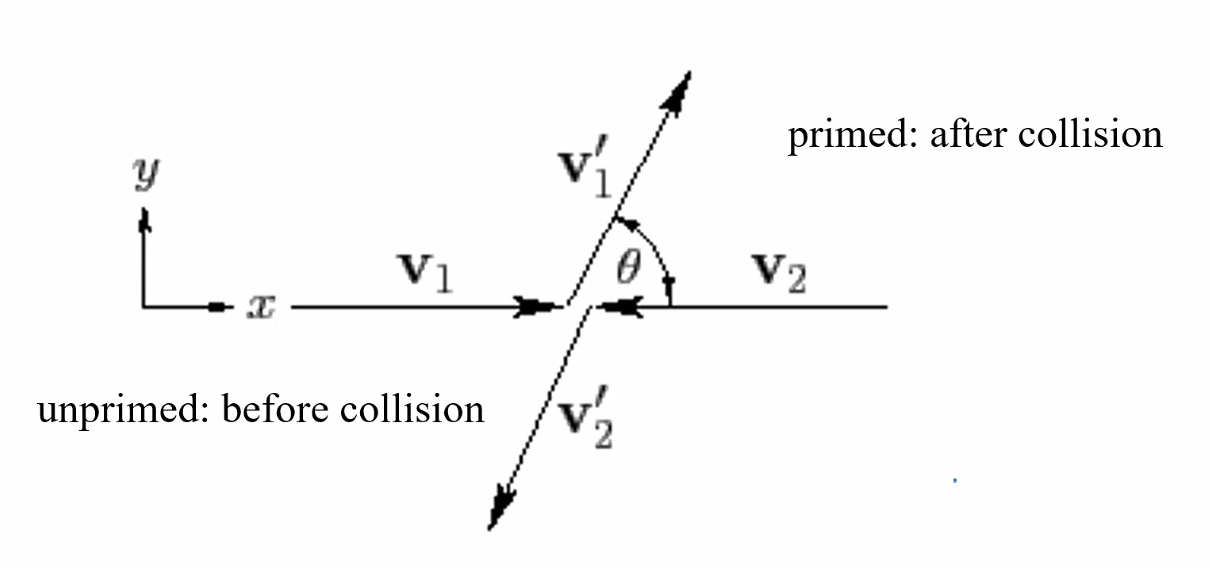
\includegraphics[scale=0.5]{Lecture-29/l29-img2.png}
\end{center}
\end{s}

\subsubsection{Differential Cross Section in COM Frame}
In the COM frame, we just find $\od{\sigma}{\Omega}$ as if a single particle of mass $\mu$ scatters off a fixed target. This is the beauty of working in the COM frame. We then have $\left(\dod{\sigma}{\Omega}\right)_{COM}$ which we must convert to the laboratory cross section. How do we do this? Consider the number of scattered particles in the center of mass frame: \[N_{sc}^{COM} = N_{inc}^{COM}\cdot \sigma_{CM}^{tot} \cdot \frac{N_{target}}{A}\]
This has to be the same in the lab frame, so:
\[N_{sc}^{COM} = N_{sc}^{lab} = N_{inc}^{lab}\cdot \sigma_{lab}^{tot}\cdot \frac{N_{target}}{A}\]
$\frac{N_{target}}{A}$ is also equal between the two expressions. Hence, we conclude that the total cross sections must be the same, that is:
\[\sigma_{COM}^{tot} = \sigma_{lab}^{tot}\]
What about the differential cross section? What must be true for the number of scattered particles in a given solid angle to be the same in the COM and lab frames?
\begin{s}
We require that $\sigma_{COM}^{tot} = \sigma_{lab}^{tot}$ so hence:
\[\left(\dod{\sigma}{\Omega}\right)_{COM}d\Omega_{COM} = \left(\dod{\sigma}{\Omega}\right)_{lab}d\Omega_{lab}\]
This can be justified as:
\[N_{sc}(\text{into $d\Omega$}) = N_{inc}\frac{N_{target}}{A}\boxed{\dod{\sigma}{\Omega}d\Omega}\]
Where the boxed expression must be the same between two cases.
\end{s}
Hence we may write:
\[\left(\dod{\sigma}{\Omega}\right)_{lab} = \left(\dod{\sigma}{\Omega}\right)_{COM} \frac{d\Omega_{COM}}{d\Omega_{lab}} = \left(\dod{\sigma}{\Omega}\right)_{COM}\abs{\frac{d\cos\theta_{COM}}{d\cos\theta_{lab}}}\]
Depicitions of the collision in the two frames is given by:
\begin{center}
    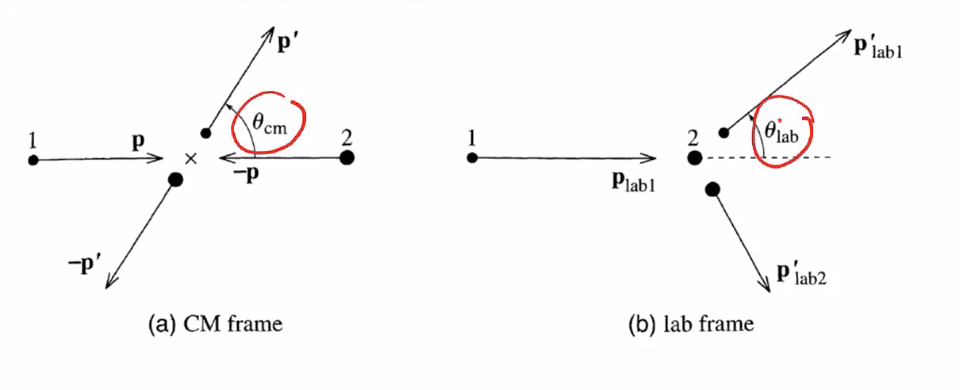
\includegraphics[scale=0.5]{Lecture-29/l29-img3.png}
\end{center}
And we want to find the relationship between the two given angles. We start with:
\[\v{p}_{COM1} = -\v{p}_{COM2} = \v{p}\]
\[\v{p}'_{COM1} = -\v{p}'_{COM2} = \v{p}'\]
By the transformation from lab to COM coordinates:
\[\v{r}_1 = \v{R} + \frac{m_2}{M}\v{r}, \quad \v{r}_2 = \v{R} - \frac{m_1}{M}\dot{\v{r}}\]
In the lab frame, particle $2$ is at rest, so:
\[\v{R} = \frac{m_1}{M}\dot{\v{r}} = \frac{\mu}{m_2}\dot{\v{r}} = \frac{\v{p}}{m_2} \]
Hence we can write:
\[\v{p}_{lab1} = m_1\dot{\v{r}}_1 = m_1\dot{\v{R}} = \mu\dot{\v{r}} = \frac{m_1}{m_2}\v{p} + \v{p}\]
Calling $\lambda = \frac{m_1}{m_2}$, we have that:
\[\v{p}_{lab1} = \lambda\v{p} + \v{p}\]
After the scattering:
\[\v{p}'_{lab1} = \lambda\v{p}' + \v{p}'\]
Drawing a picture, we know that $\v{p}'$ is just the original vector rotated by $\theta_{COM}$ on a circle. But, $\v{p}_{lab1}$ is of course larger than $\v{p}_{COM}$ (see the expression above):
\begin{center}
    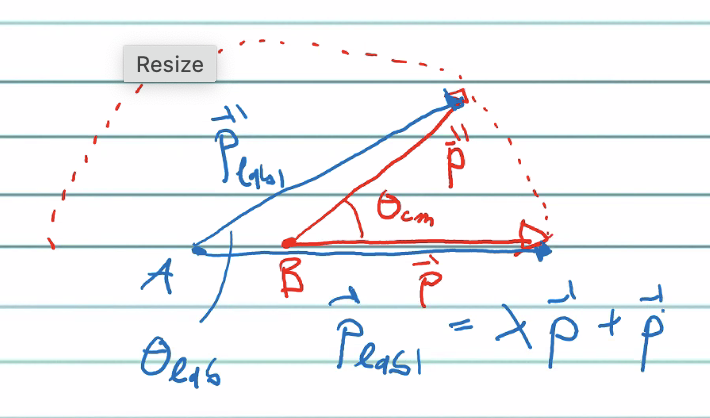
\includegraphics[scale=0.5]{Lecture-29/l29-img4.png}
\end{center}
Then using some geometry, we draw a right triangle $AFD$:
\begin{center}
    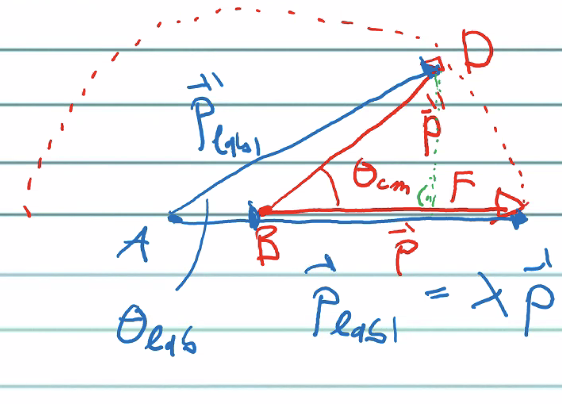
\includegraphics[scale=0.5]{Lecture-29/l29-img5.png}
\end{center}
Hence we can write (using trigonometry):
\[\tan\theta_{lab} = \frac{DF}{AF} = \frac{p\sin\theta_{COM}}{\lambda p + p\cos\theta_{COM}}\]
$p$ cancels, giving us:
\[\tan\theta_{lab} = \frac{\sin\theta_{COM}}{\lambda + \cos\theta_{COM}}\]
In the case where $m_1 = m_2$ and hence $\lambda_ = 1$, we have that:
\[\theta_{lab} = \frac{1}{2}\theta_{COM}\]
Which, returning back to the problem we wished to solve:
\[\abs{\frac{d(\cos\theta_{COM})}{d(\cos\theta_{lab})}} = \frac{(1 + 2\lambda\cos\theta_{COM} + \lambda^2)^{3/2}}{\abs{1 + \lambda \cos \theta_{COM}}} \]
The full diagram is given here:
\begin{center}
    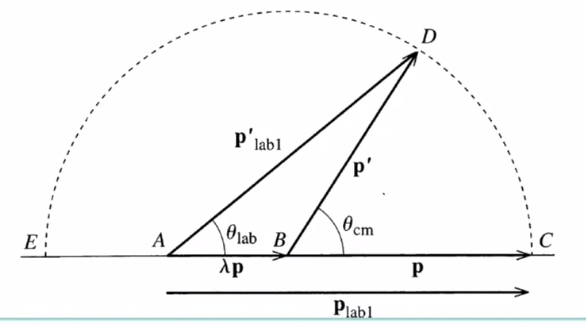
\includegraphics[scale=0.5]{Lecture-29/l29-img6.png}
\end{center}
\subsubsection{Example: Hard spheres}
Consider the example with hard spheres with $m_2 = 2m_1$. The differential cross sections can be calculated as follows:
\begin{center}
    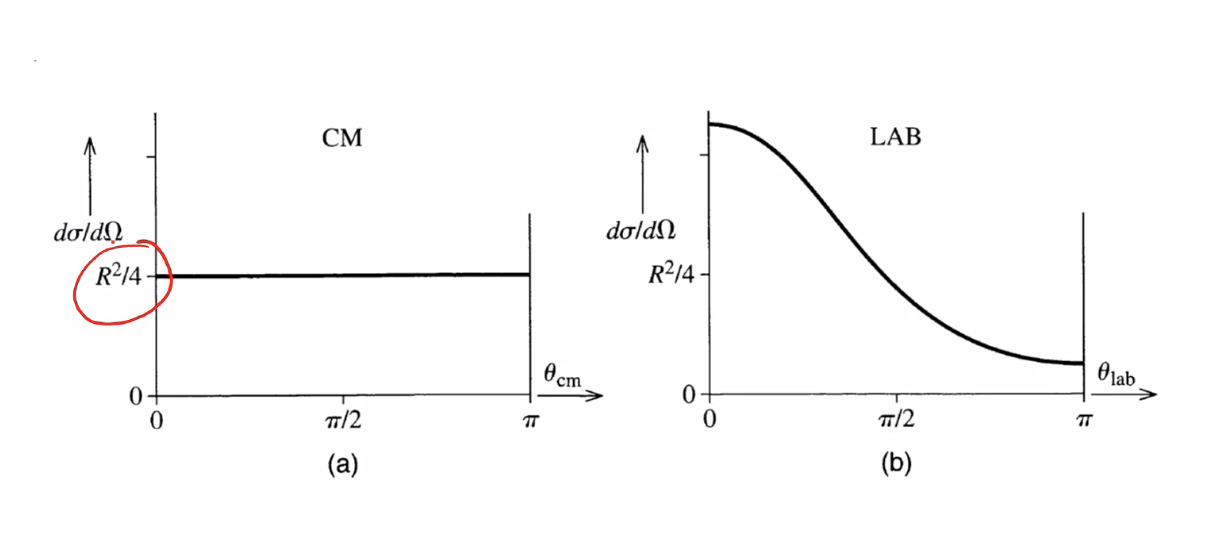
\includegraphics[scale=0.5]{Lecture-29/l29-img7.png}
\end{center}
This concludes our discussion of scattering! It was interesting to see how much a conversion to the COM frame can simplify our lives. 

\subsubsection{Coming up}
Next week, we move onto continuum mechanics, going from the discrete (photons) to waves. We recall from the HW that we could model a rope as a chain of photons, write out the coupling matrices etc. But obviously this gets very tedious and complicated if our system gets very large (we do not want to write down a coupling matrix for 1000s of masses!) Instead, we can step back and just consider the mass as a continuum, and think about the displacement of the string in space and time (the wave equation). Next week we will see how we can make the jump from the discrete masses to the continuum limit of matter, where we no longer talk about particles but macroscopic objects described by displacement fields. In doing so, we will talk about wavelike motion/standing waves, as well as other ideas that come out of this framework. It turns out that there is a lot of fundamental physics we can get to without having to know lots of microscopic information. Finally, we will end the course with nonlinear dynamics after that.